
\section*{Introduction}\label{sec:intro}

Rule-based modeling languages for molecular biology, such as Kappa
\cite{DanosEtAl-CONCUR07} and BioNetGen \cite{bngl}, or organic
chemistry, such as M{\o}d \cite{moll}, can be used to write
mechanistic models of complex reaction systems. In these approaches,
chemical transformations are represented by local graph-rewrite rules
equipped with stochastic firing rates. In a dynamical simulation,
rules induce a time series of events that might reach a state of
interest in processes like the assembly of a molecular machine, the
activation of a transcription factor, or the synthesis of a specific
chemical compound. While rule-based models provide compactness,
transparency, and the ability of handling combinatorial complexity,
the perhaps most significant advantage lies in their suitability for
causal analysis that takes into account the logically concurrent
nature of interactions.

\begin{figure}[!h]
  \vskip -0.1cm
  \begin{center}
    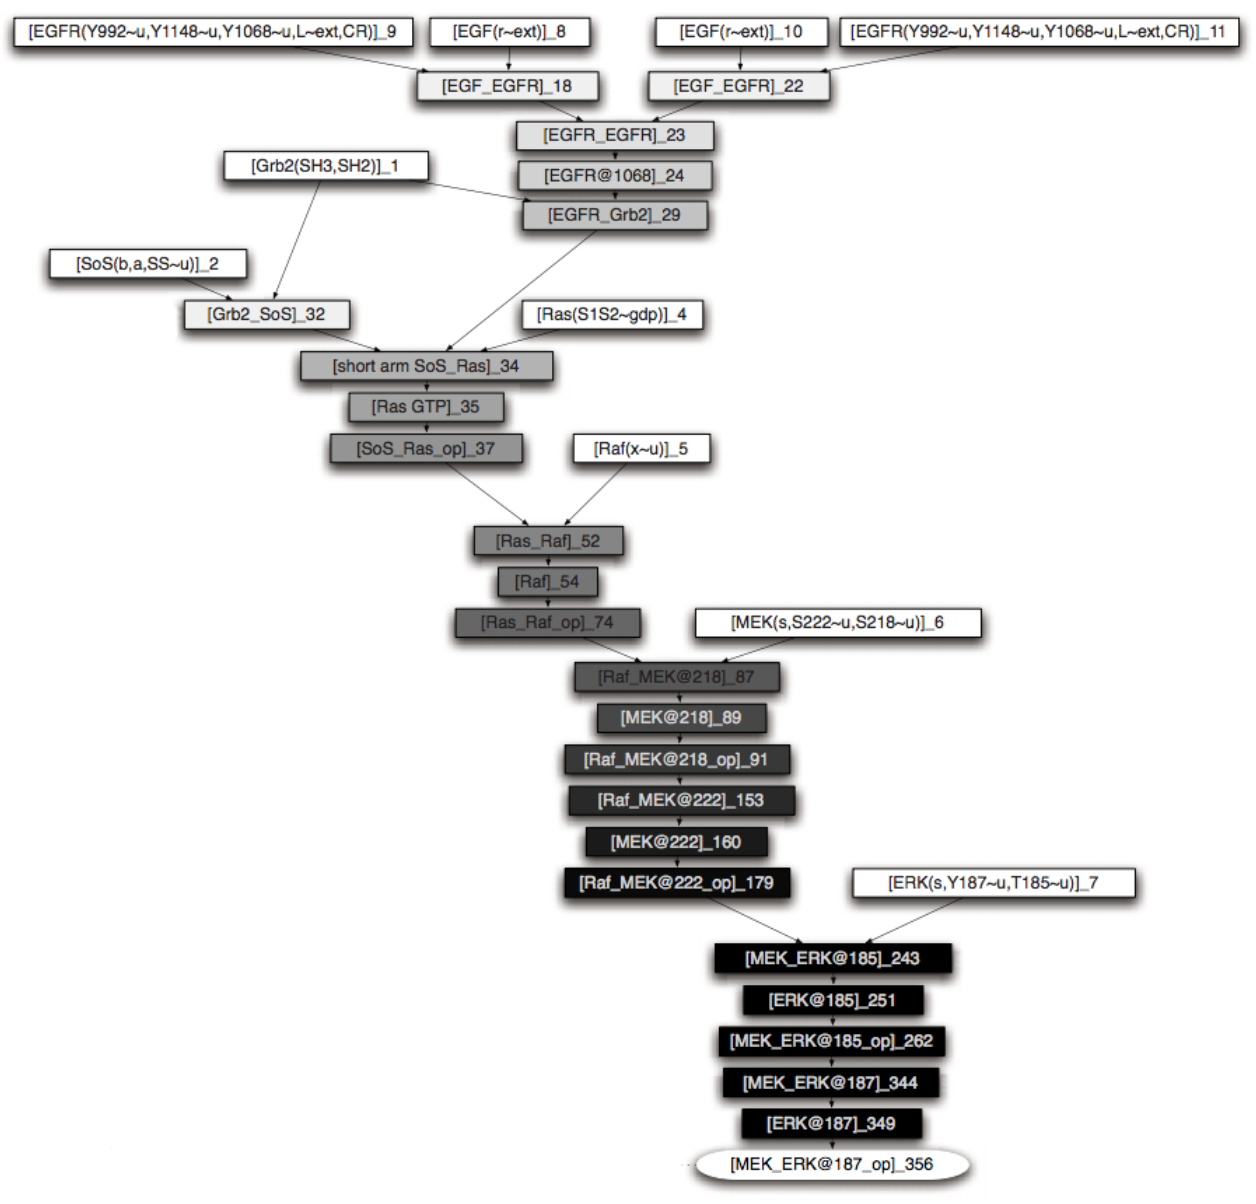
\includegraphics[scale=0.35]{figures/story-egfr.png}
  \end{center}
  \vskip -0.1cm
  \caption{An example of a story describing a part of the EGFR
    signalling pathway, adapted from
    \protect\cite{DanosEtAl-CONCUR07}. Rectangles correspond to
    individual events and solid arrows denote activation between
    them. }
  \label{fig:story-egfr}
\end{figure}


The causal analysis
\cite{DBLP:conf/fsttcs/DanosFFHH12,DanosEtAl-CONCUR07} of event series
generated by such models provides a formal definition of ``pathway"
and a means for revealing the emergence of pathways from low-level
interactions. These methods take advantage of rule structure to
\begin{inparaenum}[(i)]
\item compress a given simulation trace into a minimal subset of
  events that are necessary and jointly sufficient to replicate a
  phenomenon of interest and
\item highlight the direct causal influences between events, exposing
  the extent of concurrency.
\end{inparaenum}

% There is much more to discuss here.

We propose a distinct but complementary approach based on
\textit{counterfactual reasoning} that improves causal explanations by
\begin{inparaenum}[(i)]
\item being more sensitive to kinetics and
\item properly accounting for the causal impact from inhibition
  between events.
\end{inparaenum}